\subsection{Motivation (Vectors in 3-space)}

\begin{tcolorbox}[title=Problem 1, breakable]
    Given the point $P = (2, -1, 3)$ and the vector 
        $u = [-3, 4, 5]$, find the point $Q$
        such that $\overrightarrow{PQ} = u$.
\end{tcolorbox}

\begin{proof}
    We require $\vec{u} = [-3, 4, 5] = (q_1 - 2, q_2 - (-1), q_3 - 3)$.
    Solving componentwise, we see $(q_1, q_2, q_3) = (-1, 3, 8)$.
    Thus, $Q = (-1, 3, 8)$.
\end{proof}


\begin{tcolorbox}[title=Problem 2, breakable]
    Given the points $P(2, -1, 3)$, $Q(3, 4, 1)$,
        $R(4, -3, 4)$, $S(5, 2, 2)$. True or false (explain:)
        $PQSR$ is a parallelogram.
\end{tcolorbox}

\begin{proof}
For $PQSR$ to be a parallelogram, we require $\vec{PQ} = \vec{SR}$.
$$
\vec{PQ} = [3 - 2,\; 4 - (-1),\; 1 - 3] = [1, 5, -2]
$$
$$
\vec{SR} = [4 - 5,\; -3 - 2,\; 4 - 2] = [-1, -5, 2]
$$
Since
$$
[1, 5, -2] \neq [-1, -5, 2],
$$
it follows that $PQSR$ is not a parallelogram.
\end{proof}

\begin{tcolorbox}[title=Problem 4, breakable]
    Show that for every triple points $P, Q, R$,
        $\overrightarrow{PQ} + \overrightarrow{QR} = \overrightarrow{PR}$.
    [Method $1$: Calculate components. Method 2: Draw a picture.]
\end{tcolorbox}

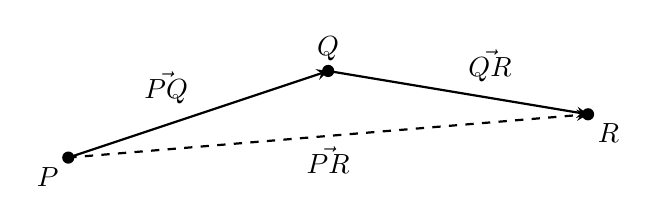
\begin{tikzpicture}[scale=1.1, >=stealth]
    % Points
    \coordinate (P) at (0,0);
    \coordinate (Q) at (3,1);
    \coordinate (R) at (6,0.5);

    % Dots
    \fill (P) circle (2pt) node[below left] {$P$};
    \fill (Q) circle (2pt) node[above] {$Q$};
    \fill (R) circle (2pt) node[below right] {$R$};

    % Vectors
    \draw[->, thick] (P) -- (Q) node[midway, above left] {$\vec{PQ}$};
    \draw[->, thick] (Q) -- (R) node[midway, above right] {$\vec{QR}$};
    \draw[->, thick, dashed] (P) -- (R) node[midway, below] {$\vec{PR}$};
\end{tikzpicture}

\subsection{$\mathbb{R}^n$ and $\mathbb{C}^n$}

\begin{tcolorbox}[title=Problem 2, breakable]
    Consider the vectors 
        $u = (2, 1)$, $v = (-5, 3)$, $w = (3, 4)$
            in $\mathbb{R}^2$.
    Do there exists real numbers $a, b$
        such that $au + bv = w$?
    What if $v = (6, 3)$.
\end{tcolorbox}

\begin{proof}
    We require $au + bv = w
    \iff a(2, 1) + b(-5, 3) = (3, 4)
    \iff (2a, a) + (-5b, 3b) = (3, 4)
    \iff (2a - 5b, a + 3b) = (3, 4)$.
    Thus
    $$
    \begin{cases}
    2a - 5b = 3 \\
    a + 3b = 4
    \end{cases}
    $$
    which has the solution $a = \frac{29}{11},\ b = \frac{5}{11}$.
    If $v = (6, 3)$, we require
    $$
    a(2, 1) + b(6, 3) = (3, 4)
        \iff (2a + 6b, a + 3b) = (3, 4).
    $$
    Thus
    $$
    \begin{cases}
    2a + 6b = 3 \\
    a + 3b = 4
    \end{cases}
    $$
    which has no solution.
    To see this has no solution, note
    $$
    a + 3b = 4 \implies 6b = 8 - 2a.
    $$
    Plugging into the first equation gives
    $$
    2a + (8 - 2a) = 3 \implies 8 = 3,
    $$
    which is a contradiction.
\end{proof}

\begin{tcolorbox}[title=Problem 3, breakable]
    Give a detailed proof of (8) of Theorem 1.2.3 (just checking!).
    [Write out all steps of the proof and give a reason for each step.]
\end{tcolorbox}

\begin{proof}
    Let $x = [x_1, x_2, \ldots, x_n] \in F^n$ be a vector and let $c, d \in F$ where $F$ is a field.  
    Then
    $$
    (cd)x = [(cd)x_1, (cd)x_2, \ldots, (cd)x_n].
    $$
    Since $F$ is a field, scalar multiplication in $F$ is associative thus
    $$
    (cd)x_i = c(d x_i) \quad \text{for each } i = 1, 2, \ldots, n.
    $$
    Therefore,
    $$
    (cd)x = [c(d x_1), c(d x_2), \ldots, c(d x_n)] = c(d x),
    $$
\end{proof}

\begin{tcolorbox}[title=Problem 4, breakable]
    In Definition 1.2.1, $n = 1$ is not ruled out.
    What do the elements of $\mathbb{R}^1$ look like?
    Describe sums and scalar multiples in $\mathbb{R}^1$.
\end{tcolorbox}

\begin{proof}
    The elements of $\mathbb{R}^1$ look like $[x_1]$ where $x_1 \in \mathbb{R}$.  
    Sums and scalar multiples behave identically to the operations in the field $\mathbb{R}$.
\end{proof}

\subsection{Vectors Spaces: The Axioms some Examples}

\begin{tcolorbox}[title=Problem 1, breakable]
    Let $V$ be a vector space over a field $F$.
    Let $T$ be a nonempty set and let $W = \mathcal{F}(T, V)$
    be the set of all functions $x : T \longrightarrow V$.
    Show that $W$ can be made into a vector space over $F$
    in a natural way. [Hint: Use the definitions in Example 1.3.4
    as a guide.]
\end{tcolorbox}

\begin{proof}
    For $x, y \in W$, $x = y$ means that $x(t) = y(t)$ for all $t \in T$.
    If $x, y \in W$ and $c \in F$, define functions $x + y$ and $cx$ by the 
    formulas $(x + y)(t) = x(t) + y(t)$ and $(cx)(t) = c x(t)$ for all $t \in T$.
    Let $\theta$ be the function defined by $\theta(t) = 0$ for all $t \in T$,
    and for $x \in W$, let $-x$ be the function defined by $(-x)(t) = -x(t)$ for 
    all $t \in T$.
\end{proof}

\begin{tcolorbox}[title=Problem 2, breakable]
    The definition of a vector space (1.3.1) can be formulated 
    as follows. A vector space over $F$ is a nonempty set $V$
    together with a pair of mappings $\sigma : V \longrightarrow V$
    and $\mu : F \times V \longrightarrow V$. ($\sigma$ suggests `sum'
    and $\mu$ suggests `multiple') having the following properties 
    $\sigma(x, y) = \sigma(y, x)$ for all $x, y \in V$;
    $\sigma(\sigma(x,y), z) = \sigma(x, \sigma(y, z))$
    for all $x, y, z \in V$ etc. The exercise: Write out the `etc.' in detail.
\end{tcolorbox}

\begin{proof}
    We list the $9$ axioms below:
    \begin{enumerate}
        \item $x,y \in V \implies \sigma(x, y) \in V$
        \item $x \in V, c \in F \implies \mu(c, x) \in V$
        \item $x, y \in V \implies \sigma(x, y) = \sigma(y, x)$
        \item $x, y, z \in V \implies \sigma(x, \sigma(y, z)) = \sigma(\sigma(x, y), z)$
        \item $\exists 0 \in V$ such that $\sigma(0, v) = v = \sigma(v, 0)$
        \item $x \in V \implies -x \in V$ such that $\sigma(x, -x) = 0 = \sigma(-x, x)$
        \item $x, y \in V$ and $c \in F \implies \mu(c, \sigma(x, y)) = \sigma(\mu(c, x), \mu(c, y))$
        \item $\exists 1 \in F$ such that $x \in V \implies \mu(1, x) = x$
        \item $a, b \in F$ and $x \in V \implies \mu(a, \mu(b, x)) = \mu(a b, x)$
    \end{enumerate}
\end{proof}

\begin{tcolorbox}[title=Problem 3, breakable]
    Let $V$ be a complex vector space (1.3.2).
    Show that $V$ is also a real vector space 
    (sums as usual, scalar multiplication restricted to real scalars).
    These two ways of looking at $V$ may be indicated by writing $V_c$ and $V_r$.
\end{tcolorbox}

\begin{proof}
    Clearly $V_r$ is closed under scalar multiplication and vector addiction
        and is a vector space.
\end{proof}

\begin{tcolorbox}[title=Problem 4, breakable]
    Every real vector space $V$ can be `embedded'
    in a complex vector space $W$ in the following way:
        let $W = V \times V$ be the real vector space 
        constructed as in example 1.3.10 and define multiplication 
        by complex scalars by the formula 
        $(a + bi)(x, y) = (ax - by, bx + ay)$
        for $a, b \in \mathbb{R}$ and $(x, y) \in W$.
    [In particular, $i(x, y) = (-y, x)$. Think of $(x, y)$ as `$x + iy$']
    Show that $W$ satisfies the axioms for a complex vector space ($W$ is 
    called the \emph{complexification} of $V$.)
\end{tcolorbox}

\begin{proof}
    Below are the 9 vector space axioms.
    \begin{enumerate}
        \item Let $x, y \in W$. 
              Then $x = (v_1, v_2), y = (w_1, w_2) \in V \times V$,
                and $(v_1, v_2) + (w_1, w_2) = (v_1 + w_1, v_2 + w_2)$. 
              Now, $v_1 + w_1 \in V$ and $v_2 + w_2 \in V$, thus $(v_1 + w_1, v_2 + w_2) \in V \times V$.
        \item Let $x \in W$ and $c \in \mathbb{C}$. 
              Then $x = (v_1, v_2) \in V \times V$, $c = a + bi \in \mathbb{C}$, and $(a + bi)(v_1, v_2) = (a v_1 - b v_2, b v_1 + a v_2)$.
              Clearly $a v_1 - b v_2 \in V$ and $b v_1 + a v_2 \in V$, thus $(a v_1 - b v_2, b v_1 + a v_2) \in V \times V$.
        \item Let $x, y \in W$. Then $x = (v_1, v_2), y = (w_1, w_2) \in V \times V$.
              Then $x + y = (v_1, v_2) + (w_1, w_2) = (v_1 + w_1, v_2 + w_2) = (w_1 + v_1, w_2 + v_2) = (w_1, w_2) + (v_1, v_2) = y + x$.
        \item Let $x, y, z \in W$. Then $x = (v_1, v_2), y = (w_1, w_2), z = (s_1, s_2) \in V \times V$.
             Then $(x + y) + z = [(v_1, v_2) + (w_1, w_2)] + (s_1, s_2) = (v_1 + w_1, v_2 + w_2) + (s_1, s_2) = ((v_1 + w_1) + s_1, (v_2 + w_2) + s_2) = (v_1 + (w_1 + s_1), v_2 + (w_2 + s_2)) = (v_1, v_2) + (w_1 + s_1, w_2 + s_2) = (v_1, v_2) + [(w_1, w_2) + (s_1, s_2)] = x + (y + z)$.
        \item Let $x \in W$. Then $x = (v_1, v_2) \in V \times V$ and $x + 0 = (v_1, v_2) + (0, 0) = (v_1 + 0, v_2 + 0) = (v_1, v_2)$.
        \item Let $x \in W$. Then $x = (v_1, v_2) \in V \times V$ and $x + (-x) = (v_1, v_2) + (-v_1, -v_2) = (v_1 - v_1, v_2 - v_2) = (0, 0) = 0 = (-v_1, -v_2) + (v_1, v_2) = (-x) + x$.
        \item Let $a + bi \in \mathbb{C}$ and $x, y \in W$. Then $(a+bi)((v_1, v_2) + (w_1, w_2)) = (a+bi)(v_1+w_1, v_2+w_2) = (a(v_1+w_1)-b(v_2+w_2), b(v_1+w_1)+a(v_2+w_2)) = (a v_1 - b v_2, b v_1 + a v_2) + (a w_1 - b w_2, b w_1 + a w_2) = (a+bi)(v_1, v_2) + (a+bi)(w_1, w_2)$.
        \item Let $a+bi, c+di \in \mathbb{C}$ and $x = (v_1, v_2) \in W$. Then $(a+bi)((c+di)(v_1, v_2)) = (a+bi)(c v_1 - d v_2, d v_1 + c v_2) = ((a c - b d)v_1 - (a d + b c)v_2, (b c + a d)v_1 + (b d + a c)v_2) = ((a+bi)(c+di))(v_1, v_2)$.
        \item Let $x = (v_1, v_2) \in W$. Then $1 \cdot (v_1, v_2) = (1 v_1 - 0 v_2, 0 v_1 + 1 v_2) = (v_1, v_2)$.
    \end{enumerate}
\end{proof}

\subsection{Vector Spaces: First Consequences of the Axioms}

\begin{tcolorbox}[title=Problem 1, breakable]
    In a vector space, \textcircled{1} $x - y = \theta$ if and only if \textcircled{2} $x = y$;  \textcircled{3} $x + y = z$
        if and only if \textcircled{4} $x = z - y$.
\end{tcolorbox}

\begin{proof}
    (\textcircled{1} $\longrightarrow$ \textcircled{2})
    Suppose $x - y = \theta \iff x + (-y) = \theta$.
    It follows that $-y = -x \iff y = x$.
    
    (\textcircled{2} $\longrightarrow$ \textcircled{1})
    Suppose $x = y \iff -x = -y$.
    Then $x + (-x) = x + (-y) = x - y = \theta$.

    (\textcircled{3} $\longrightarrow$ \textcircled{4})
    Suppose $x + y = z \iff x + y + (-y) = z + (-y) \iff x = z - y$.

    (\textcircled{4} $\longrightarrow$ \textcircled{3})
    Suppose $x = z - y \iff x + y = z - y + y \iff x + y = z$.
\end{proof}

\begin{tcolorbox}[title=Problem 2, breakable]
    Let $V$ be a vector space over a field $F$. If $x$ is a fixed nonzero vector,
    then the mapping $f : F \longrightarrow V$ defined by $f(c) = cx$ is injective.
    If $c$ is a fixed nonzero scalar, then the mapping $g : V \longrightarrow V$
    defined by $g(x) = cx$ is bijective.
\end{tcolorbox}

\begin{proof}
    Suppose $x$ is a fixed nonzero vector.
    Let $c, c' \in F$ such that $f(c) = f(c') \iff cx = c'x \iff c = c'$.
    The last step follows from Corollary 1.4.7 (ii).
    Thus $f$ is injective.
\end{proof}

\begin{proof}
    Suppose $c$ is a fixed nonzero scalar.
    The inverse function to $g(x) = cx$ is clearly $g^{-1}(x) = \frac{x}{c}$.
    Thus $g$ is bijective.
\end{proof}

\begin{tcolorbox}[title=Problem 3, breakable]
    If $V$ is a vector space and $y$ is a fixed vector, then the 
    mapping $\tau : V \longrightarrow V$ defined by $\tau(x) = x + y$
    is bijective (it is called \emph{translation} by the vector $y$).
\end{tcolorbox}

\begin{proof}
    Suppose $V$ is a vector space and $y$ is a fixed vector.
    The inverse function to $\tau(x) = x + y$ is clearly $\tau^{-1}(x) = x - y$.
    Thus $\tau$ is bijective.
\end{proof}

\begin{tcolorbox}[title=Problem 4, breakable]
    If $a$ is a nonzero scalar and $b$ is vector in the space $V$, then 
        the equation $ax + b = \theta$ has a unique solution $x$ in $V$.
\end{tcolorbox}

\begin{proof}
    Suppose $a$ is a nonzero scalar and $b$ is a vector in $V$.
    The equation $ax + b = \theta$ is equivalent to $ax = -b$.
    Multiplying both sides by $a^{-1}$ gives
    $a^{-1}(ax) = a^{-1}(-b) \iff (a^{-1} a)x = -a^{-1}b \iff x = -a^{-1}b$.
\end{proof}

\begin{tcolorbox}[title=Problem 5, breakable]
    If, in a vector space, $\theta'$ is a vector such that $0' + x = x$
        for even a single vector $x$S, then $\theta' = \theta$.
    [Hint: Add $-x$ to both sides of the equation.]
\end{tcolorbox}

\begin{proof}
    Suppose in a vector space $\theta'$ is a vector such that $\theta' + x = \theta$.
    Adding $-x$ to both sides gives $\theta' + x + (-x) = x + (-x) \iff \theta' + \theta = \theta \iff \theta' = \theta$.
\end{proof}

\subsection{Linear Combinations of Vectors}

\begin{tcolorbox}[title=Problem 1, breakable]
    Express the function $f(t) = \cos(t - \pi/3)$ as a linear combination 
    of the functions $\sin t$ and $\cos t$.
\end{tcolorbox}

\begin{proof}
    We use the standard trig identity to find 
        $f(t) = \cos(t - \pi/3) = \cos(\pi/3)\cos(t) + \sin(\pi/3)\sin(t)$.
\end{proof}

\begin{tcolorbox}[title=Problem 2, breakable]
    Express the function $e^t$ as a linear combination of the hyperbolic functions 
        $\cosh t$ and $\sinh t$.
\end{tcolorbox}

\begin{proof}
    We have the standard identity 
        $e^t = \cosh(t) + \sinh(t)$.
\end{proof}

\begin{tcolorbox}[title=Problem 3, breakable]
    Convince yourself of the correctness of the following formulas pertaining 
        to linear combinations in a vector space:
    \begin{enumerate}
        \item $c \sum_{i = 1}^n x_i = \sum_{i = 1}^{n} c x_i$.
        \item $\sum_{i = 1}^{n} a_i x_i + \sum_{i = 1}^{n} b_i x_i = \sum_{i = 1}^{n} (a_i + b_i) x_i$.
        \item $\sum_{i = 1}^{m} a_i x_I + \sum_{j = 1}^{n} b_j y_j = \sum_{k = 1}^{m + n} c_k z_k$.
                    where $c_k = a_k$ and $z_k = x_k$ for $k = 1, 2, \ldots, m$, while $c_k = b_{k - m}$ and 
                    $z_k = y_{k - m}$ for $k = m + 1, m + 2, \ldots, m + n$.
        \item \begin{align*}
            \left(\sum_{i = 1}^{m} c_i\right)\left(\sum_{j = 1}^{n} x_j\right) 
                &= \sum_{i = 1}^{m} \left(\sum_{j = 1}^{n} c_i x_j\right) \\
                &= \sum_{j = 1}^{n} \left(\sum_{i = 1}^{m} c_i x_j\right) \\
                &= \sum_{i, j} c_i x_j
        \end{align*}
    \end{enumerate}
    The last expression signifying with sum, with $mn$ terms, of the vectors $c_i x_j$
    for all possible combinations of $i$ and $j$.
\end{tcolorbox}

\begin{proof}
    I'm convinced.
\end{proof}

\begin{tcolorbox}[title=Problem 5, breakable]
    Show that in a vector space, $x - y$ is a linear combination of $x$ and $y$.
\end{tcolorbox}

\begin{proof} 
    Let $\alpha = 1$ and $\beta = -1$ and it 
        follows that $x - y = x + (-y) = \alpha x + \beta y$.
\end{proof}

\begin{tcolorbox}[title=Problem 6, breakable]
    True or false (explain): In $\mathbb{R}^3$,
    \begin{enumerate}
        \item the vector $x = (0, 6, 3)$ is a linear combination of $(2, 1, 0)$ and $(-3, 2, 0)$;
        \item the vector $x = (2, 1, -2)$ is a linear combination of $(2, 1, 0)$ and $(-3, 2, 0)$.
    \end{enumerate}
\end{tcolorbox}

\begin{proof}
    We must have
    \[
        (0, 6, 3) = \alpha(2, 1, 0) + \beta(-3, 2, 0) = (2\alpha - 3\beta, \alpha + 2\beta, 0)
    \]
    for $\alpha, \beta \in \mathbb{R}$.
    We obtain
    \begin{enumerate}
        \item $0 = 2\alpha - 3\beta$
        \item $6 = \alpha + 2\beta$
        \item $3 = 0$
    \end{enumerate}
    Since $3 \neq 0$, no solution exists.
    Now suppose
    \[
        (2, 1, -2) = \alpha(2, 1, 0) + \beta(-3, 2, 0)
        = (2\alpha - 3\beta, \alpha + 2\beta, 0).
    \]
    We obtain
    \begin{enumerate}
        \item $2 = 2\alpha - 3\beta$
        \item $1 = \alpha + 2\beta$
        \item $-2 = 0$
    \end{enumerate}
    Since $-2 \neq 0$, no solution exists. 
\end{proof}

\subsection{Linear Subspaces}

\begin{tcolorbox}[title=Problem 1, breakable]
    Let $M$ and $N$ be the subsets of $\mathbb{R}^2$
    defined as follows:
    \[M = \{(a, 0) \mid a \in \mathbb{R}\}, N = \{(0, b) \mid b \in \mathbb{R}\}\]
    Show that $M$ and $N$ are linear subspaces of $\mathbb{R}^2$
    and describe the linear subspaces $M \cap N$ and $M + N$.
\end{tcolorbox}

\begin{proof}
    First note $\theta = (0, 0) \in M, N$.
    Let $x, y \in M$ such that $x = (a_1, 0), y = (a_2, 0)$.
    Then $x + y = (a_1, 0) + (a_2, 0) = (a_1 + a_2, 0) \in M$.
    Let $c \in \mathbb{R}$.
    Then $cx = c(a_1, 0) = (c a_1, 0) \in M$.
    The argument for $N$ is the same.
    The linear subspace $M + N$ is all of $\mathbb{R}^2$,
        and the linear subspace $M \cap N$ is $\{(0, 0)\}$.
\end{proof}

\begin{tcolorbox}[title=Problem 2, breakable]
    Let $\mathcal{F} = \mathcal{R}$ as in Example 1.6.5, fix a 
        nonempty subset $T$ of $\mathbb{R}$, and let 
        \[M = \{x \in \mathcal{F} \mid x(t) = 0 \text{ for all } t \in T\}\]
        Show that $M$ is a linear subspace of $\mathcal{F}$.
\end{tcolorbox}

\begin{proof}
    Let $x, y \in M$.  
    Then for all $t \in T$, $(x + y)(t) = x(t) + y(t) = 0 + 0 = 0$, so $x + y \in M$.  
    Let $x \in M$ and $c \in \mathbb{R}$.  
    Then for all $t \in T$, $(c x)(t) = c \cdot x(t) = c \cdot 0 = 0$, so $c x \in M$.  
    Thus $M$ is a linear subspace of $\mathcal{F}$.
\end{proof}

\begin{tcolorbox}[title=Problem 3, breakable]
    With $\mathcal{F} = \mathcal{F}(\mathbb{R}$) as in 1.6.5, let 
    \[M = \{x \in \mathcal{F} \mid x = 0 \text{ on } (-\infty, 0]\}\]
    \[N = \{x \in \mathcal{F} \mid x = 0 \text{ on } (0, +\infty)\}\]
    Prove that $M + N = \mathcal{F}$ and $M \cap N = \{\theta\}$.
\end{tcolorbox}

\begin{proof}
    Let $f \in \mathcal{F}$. Define
    \[
    x(t) = 
    \begin{cases}
    f(t), & t > 0 \\[2mm]
    0, & t \le 0
    \end{cases} 
    \in M, \quad
    y(t) = 
    \begin{cases}
    f(t), & t \le 0 \\[1mm]
    0, & t > 0
    \end{cases} 
    \in N.
    \]
    Then $f = x + y$, so $M + N = \mathcal{F}$.  
    Now, let $z \in M \cap N$. Then $z(t) = 0$ for $t \le 0$ and $z(t) = 0$ for $t > 0$.  
    Thus $z = \theta$ so $M \cap N = \{\theta\}$.  
\end{proof}

\begin{tcolorbox}[title=Problem 4, breakable]
    Let $M$ and $N$ be linear subspaces of a vector space $V$, and let 
    \[M \cup N = \{x \in V \mid x \in M \text{ or } x \in N\}\]
    be the union of $M$ and $N$.
    True or false (explain): $M \cup N$ is a linear subspace of $V$.
    [If true, give a proof. If false, give a counterexample (an example of $V$, $M$, $N$
        for which $M \cup N$ is not a linear subspace of $V$).]
\end{tcolorbox}

\begin{proof}
    Let $M$ and $N$ be the subsets of $\mathbb{R}^2$
    defined as follows:
    \[
    M = \{(a, 0) \mid a \in \mathbb{R}\}, \quad N = \{(0, b) \mid b \in \mathbb{R}\}.
    \]
    We showed in Problem 1 that $M$ and $N$ are linear subspaces of $\mathbb{R}^2$.
    But notice that $(1, 0) \in M$ and $(0, 1) \in N$, yet $(1, 0) + (0, 1) = (1, 1) \notin M \cup N$.
\end{proof}

\begin{tcolorbox}[title=Problem 6, breakable]
    Let $V$ be a vector space and let $A$ be any subset of $V$.
    There exist linear subspaces of $V$ that contain $A$
    (for instance, $V$ itself is such a subspace).
    Let $\mathcal{n} = \{N \mid N  \text{ is a linear subspace of $V$ containing $A$}\}$.
    Show that $\mathcal{n}$ contains a smallest element.
    [Try $\cap \mathcal{n}$.] 
    Thus, there exists a smallest linear subpsace of $V$ containing $A$.
\end{tcolorbox}

\begin{proof}
    Let $P$ be an arbitrary linear subspace in $\mathcal{n}$.  
    Clearly, all elements in $\cap \mathcal{n}$ are in $P$, thus $\cap \mathcal{n} \subseteq P$.  
    Now, since all linear subspaces in $\mathcal{n}$ contain $0$, we have $0 \in \cap \mathcal{n}$.  
    Let $x, y \in \cap \mathcal{n}$ and $c \in F$, where $F$ is the field of scalars of $V$.  
    Let $V$ be an arbitrary element in $\mathcal{n}$.  
    Since $x, y \in \cap \mathcal{n}$, it follows that $x, y \in V$,  
    thus $x + y \in V$.  
    Therefore, $\cap \mathcal{n}$ is a linear subspace of $V$.
\end{proof}

\begin{tcolorbox}[title=Problem 7, breakable]
    Let $V$ be a vector space and let $\mathcal{n}$ be any set of linear subspaces of $V$.
    Let $A$ be the \emph{union} of the subspaces in $\mathcal{n}$, that is,
    \[A = \cup \mathcal{n} = \{x \in V \mid x \in M \text{ for some } M \in \mathcal{n}\}\]
    Apply Exercise 6 to conclude that there exists a linear subspace of $V$ that contains every $M \in \mathcal{n}$.
\end{tcolorbox}

\begin{proof}
    Clearly $\cup \mathcal{n} \subseteq V$.  Let $A = \cup \mathcal{n}$.
    By Problem 6, there exists a smallest linear subspace of $V$
    containing $A$.  Since for every $M \in \mathcal{n}$,
    $M \subseteq A$, this linear subspace contains every
    $M \in \mathcal{n}$.
\end{proof}

\begin{tcolorbox}[title=Problem 8, breakable]
    A linear subspace $M$ of a vector of a vector space $V$
    is closed under subtraction: if $x,y \in M$ then $x - y \in M$.
\end{tcolorbox}

\begin{proof}
    Suppose $x,y \in M$, where $M$ is a linear subspace of a vector space $V$.
    Let $c = -1$. Then $cy = -1 \cdot y = -y \in M$.
    Thus $x + (-y) = x - y \in M$.
\end{proof}

\begin{tcolorbox}[title=Problem 9, breakable]
    Let $V$ be a vector space and let $\mathcal{n}$ be a set of linear subspaces 
    of $V$, having the following property: if $M, N \in \mathcal{n}$ then there exists 
    $P \in \mathcal{n}$ such that $M \subset P$. (That is, any two elements of $\mathcal{n}$
    are contained in a third.) Prove that $\cup \mathcal{n}$ is a linear subspace of $V$.
\end{tcolorbox}

\begin{proof}
    Let $x,y \in \cup \mathcal{n}$ and let $c$ be a scalar of the vector space $V$.
    Then $x \in M$ for some $M \in \mathcal{n}$.
    Since $M$ is a linear subspace, $cx \in M$, thus $cx \in \cup \mathcal{n}$.
    Now $y \in N$ for some $N \in \mathcal{n}$.
    There exists $P \in \mathcal{n}$ such that
        $M \subseteq P$ and $N \subseteq P$.
    Thus $x,y \in P$.
    Since $P$ is a linear subspace, $x + y \in P$,
    thus $x + y \in \cup \mathcal{n}$.
    It follows that $\cup \mathcal{n}$ is a linear subspace of $V$.
\end{proof}

\begin{tcolorbox}[title=Problem 11, breakable]
    Let $M$ and $N$ be linear subspaces of $V$.
    Prove that the following conditions are equivalent:
    \begin{enumerate}
        \item $M \cap N = \{\theta\}$;
        \item if $y \in M$, $z \in N$ and $y + z = \theta$, then $y = z = \theta$;
        \item if $y + z = y' + z'$, where $y, y' \in M$ and $z, z' \in N$, then $y = y'$
              and $z = z'$.
    \end{enumerate}
\end{tcolorbox}

\begin{proof}
    (1 $\longrightarrow$ 2) 
    Suppose $M \cap N = \{\theta\}$.
    Furthermore, suppose $y \in M$, $z \in N$ and $y + z = \theta$.
    Then $y = -z \in M$, so $z \in M \cap N$.
    Since $M \cap N = \{\theta\}$, it follows that $z = \theta$.
    Then $y = -z = -\theta = \theta$.

    (2 $\longrightarrow$ 3) 
    Suppose that if $y \in M$, $z \in N$ and $y + z = \theta$, then $y = z = \theta$.
    Suppose $y + z = y' + z'$, where $y, y' \in M$ and $z, z' \in N$.
    Then $(y - y') + (z - z') = \theta$.
    By 2 it follows that $y - y' = \theta$ and $z - z' = \theta$,
    so $y = y'$ and $z = z'$.

    (3 $\longrightarrow$ 1) 
    Suppose that if $y + z = y' + z'$, where $y, y' \in M$ and $z, z' \in N$, then $y = y'$ and $z = z'$.
    Let $x \in M \cap N$. Then $x \in M$ and $x \in N$.
    Consider $x + \theta = \theta + x$. By 3 it follows that$x = \theta$ and $\theta = x$.
    Therefore $M \cap N = \{\theta\}$.
\end{proof}

\begin{tcolorbox}[title=Problem 12, breakable]
    Let $M$ and $N$ be linear subspaces of $V$.
    If $M + N = V$ and $M \cap N = \{\theta\}$ (cf. Exercise 11),
    $V$ is said to be the \emph{direct sum} of $M$ and $N$,
    written $V = M \oplus N$. Prove that the following conditions are 
    equivalent:
    \begin{enumerate}
        \item $V = M \oplus N$;
        \item for each $x \in V$, there exist unique elements $y \in M$
              and $z \in N$ such that $x = y + z$.
    \end{enumerate}
\end{tcolorbox}

\begin{proof}
    ($\longrightarrow$) Suppose $V = M \oplus N$.
    Let $x$ be an arbitrary element in $V$.
    Then there exists $m \in M$ and $n \in N$ such that $x = m + n$.
    Suppose there also exists $m' \in M$ and $n' \in N$ such that $x = m' + n'$.
    Then $m + n = m' + n'$.
    By Problem 11, $m = m'$ and $n = n'$,
    thus $m$ and $n$ are unique.

    ($\longleftarrow$) Suppose for each $x \in V$, there exist unique elements $y \in M$
        and $z \in N$ such that $x = y + z$.
    Let $x$ be an arbitrary element in $V$.
    Clearly $x = y + z$ where $y \in M$ and $z \in N$, thus $x \in M + N$.
    Let $x$ be an arbitrary element in $M + N$.
    Thus $x = m + n$ for some $m \in M$ and $n \in N$.
    Therefore $V = M + N$.

    Let $x \in M \cap N$.
    Then
    \[
        x = x + \theta \quad \text{with } x \in M,\ \theta \in N,
    \]
    and
    \[
        x = \theta + x \quad \text{with } \theta \in M,\ x \in N.
    \]
    Thus $x = \theta$.
    Therefore $M \cap N = \{\theta\}$.
\end{proof}

\begin{tcolorbox}[title=Problem 13, breakable]
    Let $V$ be the real vector space of all functions $x : \mathbb{R} \longrightarrow \mathbb{R}$ (1.3.4).
    Call $y \in V$ \emph{even} if $y(-t) = y(t)$ for all $t \in \mathbb{R}$, and call $z \in V$ \emph{odd}
    if $z(-t) = -z(t)$ for all $t \in \mathbb{R}$. Let 
    \[M = \{y \in V \mid y \text{ is even}\}, \quad N = \{z \in V \mid z \text{ is odd}\}.\]
    \begin{enumerate}
        \item Prove that $M$ and $N$ are linear subspaces of $V$ and that 
              $V = M \oplus N$ in the sense of Exercise 12. [Hint: If $x \in V$ consider 
              the functions of $y$ and $z$ defined by $y(t) = \frac{1}{2}[x(t) + x(-t)]$,
              $z(t) = \frac{1}{2}[x(t) - x(-t)]$].
        \item What does (i) say for $x(t) = e^t$?
        \item What does (i) say for a polynomial function $x$?
    \end{enumerate}
\end{tcolorbox}

\begin{proof}
    Clearly the zero function is in both $M$ and $N$.
    Let $x, y \in M$ and let $c \in \mathbb{R}$.
    Then $x(-t) = x(t)$ and it follows that $c x(-t) = c x(t)$, thus $c x \in M$.
    Also,
    \[
        (x + y)(-t) = x(-t) + y(-t) = x(t) + y(t) = (x + y)(t),
    \]
    thus $x + y \in M$.
    Let $a, b \in N$ and let $c \in \mathbb{R}$.
    Then $a(-t) = -a(t)$ and it follows that $c a(-t) = -c a(t)$, thus $c a \in N$.
    Also,
    \[
        (a + b)(-t) = a(-t) + b(-t) = -a(t) - b(t) = -(a + b)(t),
    \]
    thus $a + b \in N$.
    It follows that $M$ and $N$ are linear subspaces of $V$.
\end{proof}

\begin{proof}
    Let $x \in V$ be arbitrary. Define functions $y$ and $z$ by
    \[
    y(t) = \frac{1}{2}\big[x(t) + x(-t)\big], \qquad
    z(t) = \frac{1}{2}\big[x(t) - x(-t)\big].
    \]
    Notice
    \[
    y(-t) = \frac{1}{2}\big[x(-t) + x(t)\big] = y(t),
    \]
    so $y$ is even and thus $y \in M$.
    Also
    \[
    z(-t) = \frac{1}{2}\big[x(-t) - x(t)\big] = -\frac{1}{2}\big[x(t) - x(-t)\big] = -z(t),
    \]
    so $z$ is odd and thus $z \in N$.
    Now, for all $t \in \mathbb{R}$,
    \[
    y(t) + z(t)
    = \frac{1}{2}\big[x(t) + x(-t)\big] + \frac{1}{2}\big[x(t) - x(-t)\big]
    = x(t).
    \]
    Thus $x = y + z$ and therefore $V = M + N$.
    Suppose $x \in M \cap N$. Then $x$ is both even and odd and
    \[
    x(t) = x(-t) \quad \text{and} \quad x(t) = -x(-t).
    \]
    Thus $x(t) = -x(t)$ for all $t$, $x(t) = 0$ for all $t$.  
    Thus $M \cap N = \{\theta\}$.
    Therefore $V = M \oplus N$.
\end{proof}


\textbf{Solution (2):}
It says that $e^t$ can be written uniquely as the sum of an even function and an odd function.

\textbf{Solution (3):}
It says that any polynomial function can be written uniquely as the sum of an even polynomial and an odd polynomial.

\begin{tcolorbox}[title=Problem 16, breakable]
    Let $V$ and $W$ be vector spaces over the same field $F$ and let $V \times W$ 
        be the product vector space (1.3.11). If $M$ is a linear subspace of $V$,
        and $N$ is a linear subspace of $W$, show that $M \times N$ is a linear subspace 
        of $V \times W$.
\end{tcolorbox}

\begin{proof}
    Suppose $M$ is a linear subspace of $V$ and $N$ is a linear subspace of $W$.
    Let $x, y \in M \times N$ and let $c$ be a scalar from the field $F$.
    Then $x = (m_1, n_1)$ and $y = (m_2, n_2)$ are elements of $M \times N$, and
        $cx = c(m_1, n_1) = (c m_1, c n_1)$.
    Now, $c m_1 \in M$ and $c n_1 \in N$, thus $cx \in M \times N$.
    Also $x + y = (m_1, n_1) + (m_2, n_2) = (m_1 + m_2, n_1 + n_2)$.
    Since $m_1 + m_2 \in M$ and $n_1 + n_2 \in N$, it follows that $x + y \in M \times N$.
    Since $(\theta_V, \theta_W) \in M \times N$, it follows that $M \times N$ is a linear subspace of $V \times W$.
\end{proof}

\begin{tcolorbox}[title=Problem 17, breakable]
    If $V = V_1 \times V_2$ (1.3.11), $M_1 = \{(x_1, \theta) \mid x_1 \in V_1\}$
    and $M_2 = \{(\theta, x_2) \mid x_2 \in V_2\}$, then $V = M_1 + M_2$ and $M_1 \cap M_2 = \{\theta\}$
    (where $\theta$ stands for the zero vector of all vector spaces in sight). In the terminology
    of Exercise 12, $V$ is the direct sum of its subspaces in $M_1$ and $M_2$, that is, 
    $V = M_1 \oplus M_2$. (Generalization?)
\end{tcolorbox}

\begin{definition}
    If $V = V_1 \times V_2 \times \cdots \times V_n$, and
    \begin{enumerate}
        \item $M_1 = \{(x_1, \theta_2, \ldots, \theta_n) \mid x_1 \in V_1\}$
        \item $M_2 = \{(\theta_1, x_2, \ldots, \theta_n) \mid x_2 \in V_2\}$
        \item $\ldots$
        \item $M_n = \{(\theta_1, \theta_2, \ldots, x_n) \mid x_n \in V_n\}$
    \end{enumerate}
    then $V$ is the direct sum of its subspaces $M_1, M_2, \ldots, M_n$, or
    \[
        V = M_1 \oplus M_2 \oplus \cdots \oplus M_n.
    \]
\end{definition}

\begin{tcolorbox}[title=Problem 18, breakable]
    Let $M$ and $N$ be linear subspaces of $V$ whose union $M \cup N$
        is also a linear subspace. Prove that either $M \subset N$
        or $N \subset M$.
    [Hint: Assume to the contrary that neither of $M, N$ is contained in the other;
        choose vectors $y \in M$, $z \in N$ with $y \notin N$, $z \notin M$ and try to find 
        a home for $y + z$.]
\end{tcolorbox}

\begin{proof}
    Let $y \in M$ and $z \in N$ such that $y \notin N$ and $z \notin M$.
    Then $y \in M \cup N$ and $z \in M \cup N$.
    Since $M \cup N$ is a linear subspace, $y + z \in M \cup N$.
    Without loss of generality, suppose $y + z \in M$.
    Then $-y \in M$ by Problem 8.
    Since $M$ is closed under addition $y + z + (-y) = z \in M$
        which is a contradiction.
\end{proof}